\documentclass[10pt,a4paper]{article}
\usepackage{graphicx}
\usepackage{mathtools}
\usepackage{xfrac}
\usepackage{amsmath, amssymb}
\usepackage{listings}
\usepackage{float}
\usepackage{wrapfig}
\usepackage{tikz}
\usepackage{fullpage}
\usepackage{hyperref}
\usepackage{mathalpha}
\usepackage{tikz}
\usepackage{cite}
\usepackage{amsthm}
\usepackage{natbib}
\usepackage{multirow}
\usepackage[T1]{fontenc}
\usepackage[a4paper, total={7in, 10.4in}]{geometry}
\usepackage{braket}

\newtheorem{theorem}{Proposition}[section]
\newtheorem{corollary}{Corollary}[theorem]
\newtheorem{lemma}[theorem]{Lemma}

\theoremstyle{definition}
\newtheorem{definition}{Definition}[section]

\theoremstyle{remark}
\newtheorem*{remark}{Remark}
\newtheorem*{example}{Example}
\newtheorem*{notation}{Notation}

\title{Numerical Solution of the Time-Independent 1D Schr\"{o}dinger Equation}
\author{David Lawton\\
        22337087}
\date{18th Dec. 2024.}

\begin{document}

\maketitle

\tableofcontents
\addcontentsline{toc}{section}{\numberline{}Abstract}
\begin{abstract}
This experiment examined a particle inside two potential wells, the infinite square well (Eq. \ref{eq: square_well}) and the harmonic potential inside the infinite square well (Eq. \ref{eq: harmonic_potential}). The time-independent Schr\"{o}dinger equation (Eq. \ref{eq: non_dim_schrodinger}) was solved using a finite difference method, and the energy eigenvalues were found using the shooting method (\ref{sec: shooting_method}). The results agreed with analytic solutions found in \ref{sec: analytic_solution}, eg. $\varepsilon_1 = -0.9506519\approx -0.9505531$, the latter of which is the analytic value. Another example being the agreement of uncertainties with analytically found values (figure \ref{fig: square_well_results}). Each $\psi_n(\tilde{x})$ was normalised, and the uncertainty principle was found to be obeyed for both potentials.\\
\indent For the harmonic potential, it was observed that the particle transitions from a harmonic oscillator to a free particle in an infinite square well, for $\varepsilon > 1$. This can be extrapolated from the change in differences between subsequent energy values, as seen in the lower left plot of figure \ref{fig: harmonic_potential_results}. The wavefunctions for the harmonic potential, which are similar to the hermite polynomials, for smaller energies, were plotted in figure \ref{fig: harmonic_potential_wavefunctions}.
\end{abstract}


\section{Background \& Theory}
In this computational laboratory, we shall be solving the time-independent Schr\"{o}dinger equation for a particle in a one-dimensional potential well. The time-independent Schr\"{o}dinger equation is 
\begin{equation}
    -\frac{\hbar^2}{2m}\frac{\mathrm{d}^2\psi(x)}{\mathrm{d}x^2} + V(x)\psi(x) = E\psi(x)
\end{equation}
where $\psi(x)$ is the wavefunction of the particle, $V(x)$ the potential the particle is under, $m$ the mass of the particle, $E$ the energy of the particle and $\hbar$ the reduced Planck constant. In this lab, we shall remove the dimensions from this equation, to avoid computation of excessively small numbers. Thus, we get the non-dimensional Schr\"{o}dinger equation. This is given by the following in the region where the potential is finite ($\tilde{x}\in (0,1)$), and $\psi(\tilde{x}) = 0$ elsewhere
\begin{equation}
    \label{eq: non_dim_schrodinger}
    \frac{\mathrm{d}^2\psi(\tilde{x})}{\mathrm{d}\tilde{x}^2} + \gamma^2(\varepsilon-\nu(\tilde{x}))\psi(\tilde{x}) = 0
\end{equation}
where our non dimensional constants, variables and functions are $\tilde{x} = x/L$, $\varepsilon = E/V_0$, $\nu(\tilde{x}) = V(\tilde{x})/V_0$ and 
\begin{equation}
    \gamma^2 = \frac{2mL^2V_0}{\hbar^2}
\end{equation}
\subsection{Analytic Solution of non-dimensional Schr\"{o}dinger Equation}
\label{sec: analytic_solution}
Our first task is to solve the non-dimensional Schr\"{o}dinger equation analytically, so that we can later verify our computational results. We must solve for the potential well defined by
\begin{equation}
    \label{eq: square_well}
    \nu(\tilde{x}) = 
        \begin{cases}
            -1 & \text{ if } 0<\tilde{x}<1\\
            \infty & \text{ otherwise}
        \end{cases}
\end{equation}
To do this we first write our non-dimensional Schr\"{o}dinger equation
\begin{equation}
    \frac{\mathrm{d}^2\psi(\tilde{x})}{\mathrm{d}\tilde{x}^2} + \gamma^2(\varepsilon+1)\psi(\tilde{x}) = 0
\end{equation}
since $\varepsilon$ has no $\tilde{x}$ dependence, the solution is simply 
\begin{equation}
    \psi(\tilde{x}) = 
        \begin{cases}
            Ae^{ik\tilde{x}} + Be^{-ik\tilde{x}} & \text{ if }x\in(0,1)\\
            0 & \text{ otherwise}
        \end{cases}
\end{equation}
where $k = \gamma\sqrt{\varepsilon+1}$. We let $\psi_M(\tilde{x}) = \psi(\tilde{x})$ for $x\in (0,1)$. Then, since $\psi$ must be smooth, we can say $\psi(0)=\psi(1)=0$. This gives us $A+B=0$, so $A=-B$. Thus we have
\begin{equation}
    \psi_M(\tilde{x}) = A(e^{ik\tilde{x}}-e^{-ik\tilde{x}}) = 2iA\sin(k\tilde{x}) = C\sin(k\tilde{x}).
\end{equation}
We then use our second boundary condition, at $\tilde{x}=1$, giving us $\sin(kx) = 0$. This gives us $k_n = n\pi$ for $n\in\mathbb{N}$. To find the solutions we then normalise the wavefunction (integrate $|\psi|^2$ and equate to 1), giving us $C=\sqrt{2}$. Thus we have our analytic solutions
\begin{equation}
    \psi_n(\tilde{x}) = \sqrt{2}\sin(n\pi\tilde{x})
\end{equation}
from our equivalent $k_n$ definition we solve for our energy values $\varepsilon_n$,
\begin{equation}
    \varepsilon_n = \frac{n^2\pi^2}{\gamma^2}-1
\end{equation}
The analytic solutions found were in agreement with those found by F. Marsiglio, University of Alberta in \cite{article}, where the later case of the harmonic oscillator embedded in the square well is also discussed. Griffith's Quantum Mechanics \cite{Griffiths_Schroeter_2018} was used as a reference for the infinite square well potential.
\subsection{Discretization, Finite Difference Method}
\label{sec: discretization,finite_diff}
To find a numerical solution for this equation, we first discretize our continuous coordinate $\tilde{x}$ and wavefunction $\psi(\tilde{x})$ into $N$ points. Thus each point is defined by $\tilde{x}_n = \frac{n}{N}$, $n = 0, 1, ..., N$. To discretize our wavefunction, we Taylor expand $\psi(\tilde{x}\pm l), l=1/(N-1)$ about $\tilde{x}$ up to fourth order, and adding the two expansions. We then act on the schrodinger equation with $ 1 + \frac{l^2}{12}\frac{\mathrm{d}^2}{\mathrm{d}\tilde{x}^2}$. Combining the resulting equations, we get
\begin{equation}
    \psi_{n+1} = \frac{2(1-\frac{5}{12}l^2k_n^2)\psi_n - (1 + \frac{1}{12}l^2k_{n-1}^2)\psi_{n-1}}{1+\frac{1}{12}l^2k_{n+1}^2}
\end{equation}
where $k_n = \gamma\sqrt{\varepsilon-\nu(\tilde{x}_n)}$. Then, by setting the first two points, we can solve for the rest of the wavefunction, given a trial energy. We can then use the Shooting Method to find the nearest higher energy which agrees with the boundary conditions.
\subsection{Shooting Method}
\label{sec: shooting_method}
The shooting method is used here to find the energy eigenvalues of the system. Using the finite difference method described, one can find the final value, $\psi_N$ for a given energy. The method adds to the energy by some $\delta\varepsilon>0$ until the final value changes sign, and then multiplies $\delta\varepsilon$ by $\sfrac{-1}{2}$ and continues. This is repeated until some specified tolerance is reached. The resulting $\varepsilon$ value is then an eigenvalue of the system.
\subsection{Uncertainty Principle}
\label{sec: uncertainty_principle}
The uncertainty principle for the dimensionless simply states, for dimensionless position and momentum operators $\tilde{x}$ and $\tilde{p}$, that
\begin{equation}
    \sigma_{\tilde{x}}\sigma_{\tilde{p}} \geq \frac{1}{2}
\end{equation}
where $\sigma_{\tilde{x}}$ and $\sigma_{\tilde{p}}$ are the standard deviations of the position and momentum. These are defined as
\begin{equation}
    \sigma_{\tilde{x}} = \sqrt{\langle\tilde{x}^2\rangle - \langle\tilde{x}\rangle^2},\quad \sigma_{\tilde{p}} = \sqrt{\langle\tilde{p}^2\rangle - \langle\tilde{p}\rangle^2}
\end{equation}
theses can be calculated from the wavefunction $\psi(\tilde{x})$ as
\begin{align}
    \braket{\tilde{x}^n} &= \int_{-\infty}^{\infty}\tilde{x}^n|\psi(\tilde{x})|^2\mathrm{d}\tilde{x}\\
    \braket{\tilde{p}^n} = \int_{-\infty}^{\infty}\tilde{p}^n&|\psi(\tilde{x})|^2\mathrm{d}\tilde{x} = (-i)^n\int_{-\infty}^{\infty}\frac{\partial^n\psi(\tilde{x})}{\partial\tilde{x}^n}\psi(\tilde{x})\mathrm{d}\tilde{x}
\end{align}
\section{Methodology}
The procedure for this experiment begins by initialising constants, such as the number of points $N$, some $\gamma^2$ value and the potential well $\nu(\tilde{x})$, as well as the array of $\tilde{x}$ values and the initial empty array of $\psi_i$ values.
\subsection{Finite Difference Method}
The first section of the experiment is to define and use the finite difference method, as in \ref{sec: discretization,finite_diff}.
\begin{lstlisting}[language=Python]
    # Define iterative method for solving the Schrodinger equation
    def iterative_method(Psi_, k_squared_vals_, N_):
        l_squared = (1/N)**2
        p_vals, q_vals = 1-(5/12)*l_squared*k_squared_vals_, \
                        1+(1/12)*l_squared*k_squared_vals_
        for i in range(2, N_):
            Psi_[i] = (2*p_vals[i-1]*Psi_[i-1] - q_vals[i-2]*Psi_[i-2])/q_vals[i]
        return Psi_
\end{lstlisting}
We write a function to, for a given energy $\varepsilon$, find the wavefunction $\psi(\tilde{x})$, using the described iterative method, and plot it. The below sample is the most important section of the function \texttt{`analysis\_no\_plot'} which is included in the function \texttt{`Shooting\_method'}.
\begin{lstlisting}[language=Python]
    # Calculate the potential and k squared values from the inputted potential.
    # points and energy.
    potential_vals = [nu_(x) for x in xtilde_vals_]
    k_squared_vals = GammaSquare_ * (nrg_vals - potential_vals)

    # For nu=-1, first two points given by
    Psi_trial[0], Psi_trial[1] = 0, 1E-4

    # Calculate the wavefunction from these points.
    Psi_trial = iterative_method(Psi_trial, k_squared_vals, N_)
\end{lstlisting}
Here, \texttt{`GammaSquare\_'} takes some value of $\gamma^2$, \texttt{`nu\_(x)'} is a specified dimensionless potential function, and  \texttt{`nrg\_vals'} is a $1\times N$ numpy array with each entry being the same trial energy value.
\subsection{Shooting Method}
\label{sec: shooting_method implementation}
In this section, the shooting method described in \ref{sec: shooting_method} is implemented, from educated starting guesses for the energy eigenvalues. The eigenvalues are recorded and the wavefunction is plotted for each eigenvalue.
\begin{lstlisting}[language=Python]
    def Shooting_method(nrg_, nu_, xtilde_vals_, N_, GammaSquare_):
        dnrg = 1E-2
        tolerance = 1E-15

        Psi_ = np.zeros(N_)
        Psi_ = analysis_no_plot(Psi_, nrg_, nu_, xtilde_vals_, N_, GammaSquare_)
        Psi_end_vals = [Psi_[-1]]

        while np.abs(dnrg) > tolerance:
            nrg_ += dnrg
            Psi_prime = analysis_no_plot(Psi_, nrg_, nu_, xtilde_vals_, N_, GammaSquare_)
            Psi_end_vals.append(Psi_prime[-1])
            if Psi_end_vals[-1]*Psi_end_vals[-2] < 0:
                dnrg = -dnrg/2
        return nrg_
\end{lstlisting}
The values for the eigenvalues $\varepsilon_i$ of the dimensionless Schr\"{o}dinger equation which we find are then compared to the analytic solutions, so that the accuracy of the method can be verified. We also experiment with varying values of initial $\delta\varepsilon$ and tolerance to see how they affect the accuracy and efficiency of the method.\\
\subsection{Normalisation and Uncertainty Principle}
\indent Of course one essential property of the wavefunction is that its square $|\psi(\tilde{x})|^2$ is normalised. To check this we simply integrate the region of non-zero values, and check that the result is 1. If an inputted wavefunction is not normalised, we can normalise it by dividing by the square root of the integral of the square of the wavefunction. It is of course easy to see here, from the analytic solution, that any wavefunction produced is in the space of square integrable functions and is not identically zero, and so is normalisable.
\indent Now that we have normalised eigenfunctions of the time-independent Schr\"{o}dinger equation, which agree with the boundary conditions, we can test that these obey the Uncertainty Principle, outlined in \ref{sec: uncertainty_principle}. We can do this by calculating the required means of $\tilde{x}, \tilde{p}$ and their squares. The standard deviation of position can be calculated simply using a function which calculates the $n$th moment of $\psi$, $\braket{\tilde{x}^n}$,
\begin{lstlisting}[language=Python]
    def expectation_value_moment(Psi_, xtilde_vals_, N_, n):
    return simps((Psi_ **2) * (xtilde_vals_**n), xtilde_vals_, dx=1/N_)
\end{lstlisting}
where simps is simply a numerical integration function, using Simpson's rule. The standard deviation of position is then calculated using a five point central difference method for the derivatives of $\psi(\tilde{x})$, and the equations for the expectation values of $\tilde{p}^n$ in \ref{sec: uncertainty_principle}. 
\begin{lstlisting}[language=Python]
    def expectation_value_p(Psi_, xtilde_vals_, N_):
        q = 0 - 1j
        dPsidx = five_point_central_difference_method(Psi_, N_)
        expec_p = q*simps(Psi_*dPsidx, xtilde_vals_, dx=1/N_)
        if np.isclose(expec_p.imag, 0, atol=1E-2):
            expec_p = 0
        return expec_p

    def expectation_value_p_squared(Psi_, xtilde_vals_, N_):
        dPsidx = five_point_central_difference_method(Psi_, N_)
        d2Psidx2 = five_point_central_difference_method(dPsidx, N_)
        return -simps(Psi_*d2Psidx2, xtilde_vals_, dx=1/N_)
\end{lstlisting}
while the five-point central difference method would mean that the derivative would not be defined at the first and last two points, we used forward and backward difference methods for these points. The standard deviation of momentum is then calculated using these expectation values. We can then check that the uncertainty principle is obeyed.
\subsection{Harmonic Potential}
Since the code for the previous sections has been written in a general fashion, not specified to the infinite square well potential, it can be repurposed for any other potential inside this well. The potential used in this section is then a harmonic potential bounded inside a potential well, defined by
\begin{equation}
    \label{eq: harmonic_potential}
    \nu(\tilde{x}) = \begin{cases}
        8(\tilde{x}-0.5)^2 - 1 & \text{ if } 0<\tilde{x}<1\\
        \infty & \text{ else}
    \end{cases}
\end{equation}
We implement the same code as before, with a different $\gamma = 1000$. However, since there is no analytic solution for this potential, instead of making educated guesses, we find energy eigenvalues by starting just above the minimum energy and implementing the shooting method as before, using the same iterative method. Once a sufficiently accurate result is reached, we record the energy, and then increase the energy by some small amount and repeat the process. This is repeated for ten energy values, and the wavefunctions are normalised and plotted. We also check the uncertainty principle, as before and plot the change between subsequent energies.
\section{Results}
\subsection{Infinite Square Well}
\label{sec: square_well_results}
The first result corresponding to the infinite square well potential is the energy eigenvalues found by the shooting method. Below in figure \ref{fig: square_well_results}, these are compared to the analytic values as derived in \ref{sec: analytic_solution}. Clearly the results are reasonably accurate, and any error can be attributed to a combination of finite difference methods in the discretization of $\psi$, and the assumption, $\psi(l)=10^{-4}$. As is clear in the upper right plot in \ref{fig: square_well_results}, the solutions are of the form $\psi_n(\tilde{x})=A\sin(n\pi \tilde{x})$ where $n$ corresponds to the $n$th energy level, as in the analytic solution. Note also, in the lower right plot in figure \ref{fig: square_well_results}, that all of the wavefunctions have the same amplitude, which we can find analytically to be $\sqrt{2}$, which clearly agrees approximately with the amplitude in the plot.\\
\indent The next result, for the square well, is that of the uncertainty principle. As can be seen in the lower centre plot in figure \ref{fig: square_well_results}, the computed values of $\sigma_{\tilde{x}}\sigma_{\tilde{p}}$ agree with the analytic values, and for all $n$, $\sigma_{\tilde{x}}\sigma_{\tilde{p}}\geq \frac{1}{2}$, as expected.\\
\indent It is also notable that when implementing the shooting method, the choice of initial $\delta\varepsilon$ was irrelevant, as long as it was less than the minimum difference between two energy levels, $1$. The results of this experiment could be improved by using a larger number of points, $N$, a higher order finite difference method, or a more informed guess of the first point of the wavefunction, $\psi(l)$.\\ 


\begin{figure}[h]
    \begin{tabular}{p{0.25\textwidth}p{0.75\textwidth}}
        \begin{tabular}{|p{0.014\textwidth}|p{0.1\textwidth}|p{0.1\textwidth}|}
            \hline
            $n$&Analytic $\varepsilon_n$&Comp. $\varepsilon_n$\\
            \hline
            1 & -0.9506519 & -0.9505531\\
            2 & -0.8026079 & -0.8022125\\
            3 & -0.5558678 & -0.5549782\\
            4 & -0.2104316 & -0.2088501\\
            5 & 0.2337005 & 0.2361716\\
            6 & 0.7765287 & 0.7800871\\
            7 & 1.4180530 & 1.4228964\\
            8 & 2.1582734 & 2.1645994\\
            9 & 2.9971897 & 3.0051961\\
            10 & 3.934802 & 3.9446866\\
            \hline
        \end{tabular}&
            \begin{tabular}{cc}
                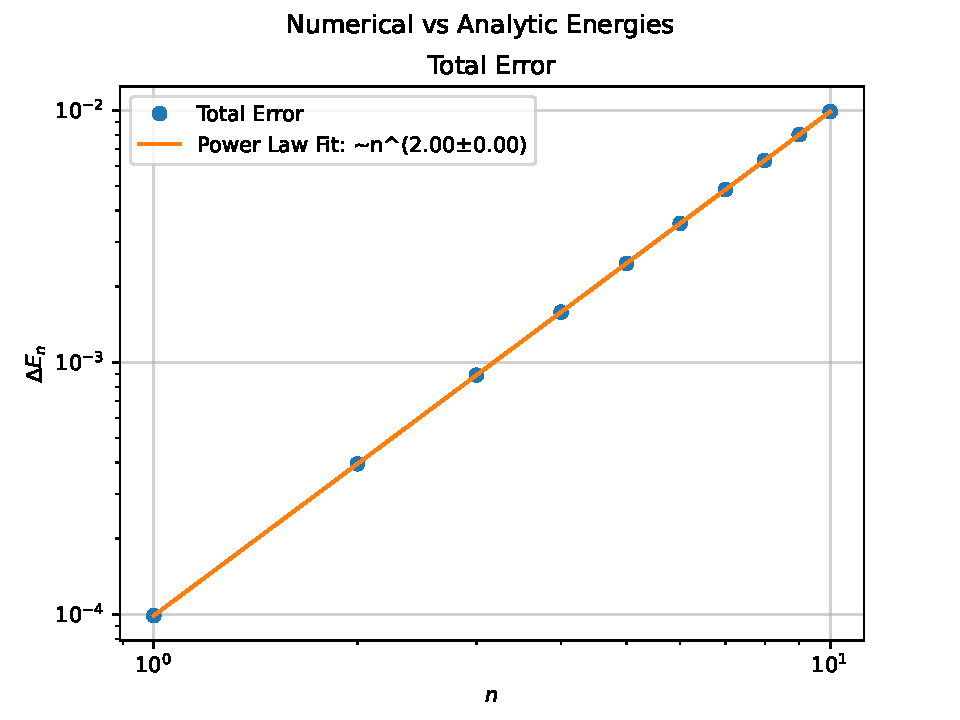
\includegraphics[width=0.38\textwidth]{energy_error_nu.pdf} &
                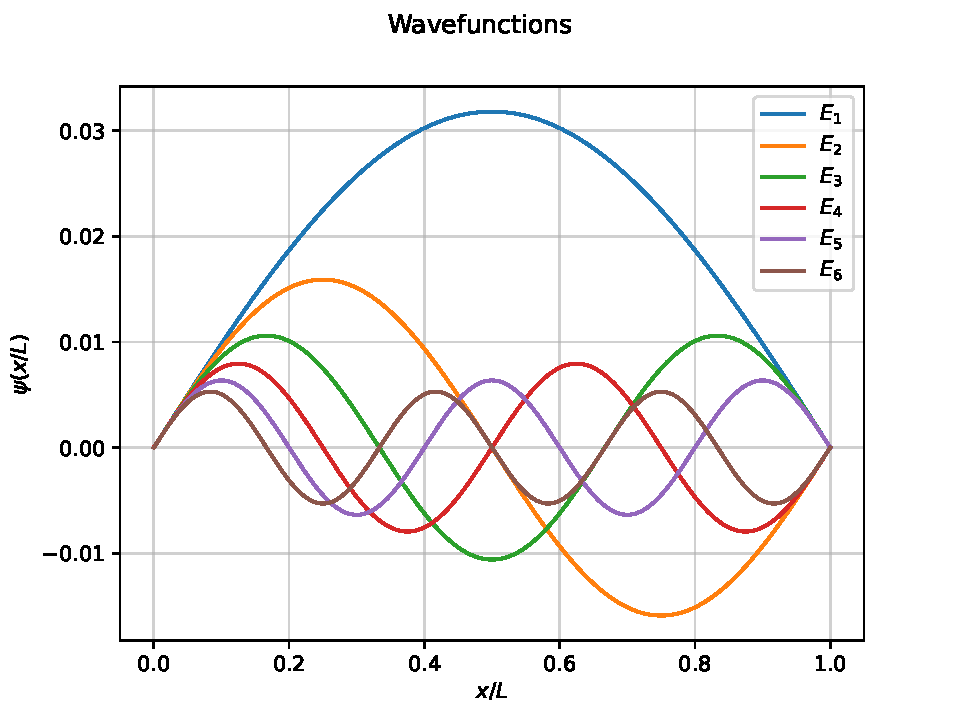
\includegraphics[width=0.38\textwidth]{wavefunctions_nu.pdf}\\
                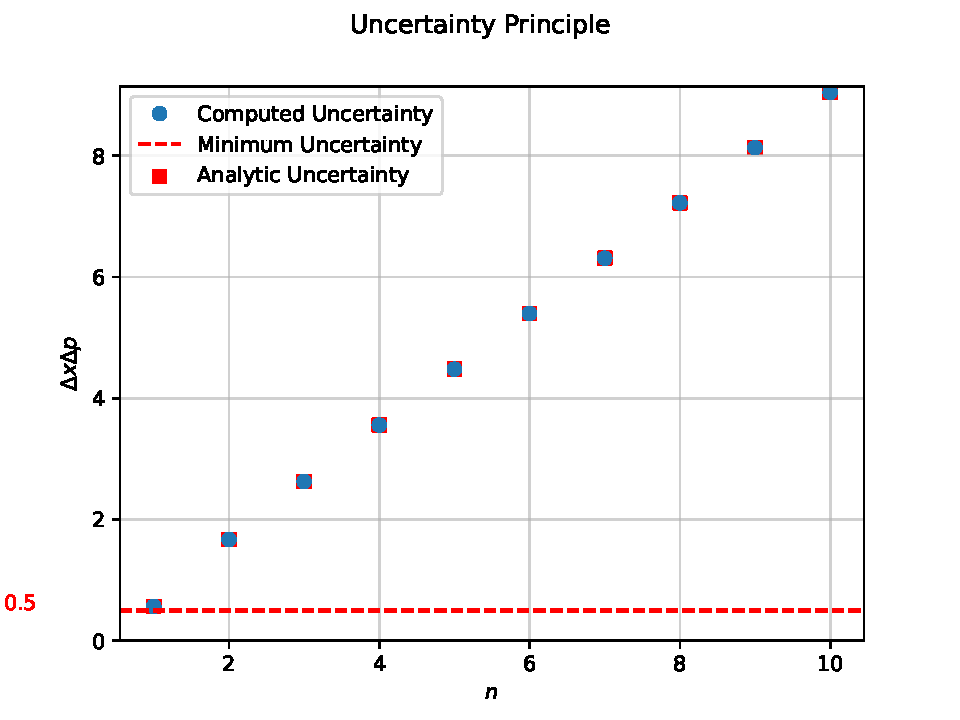
\includegraphics[width=0.38\textwidth]{uncertainty_principle_for_nu.pdf} &
                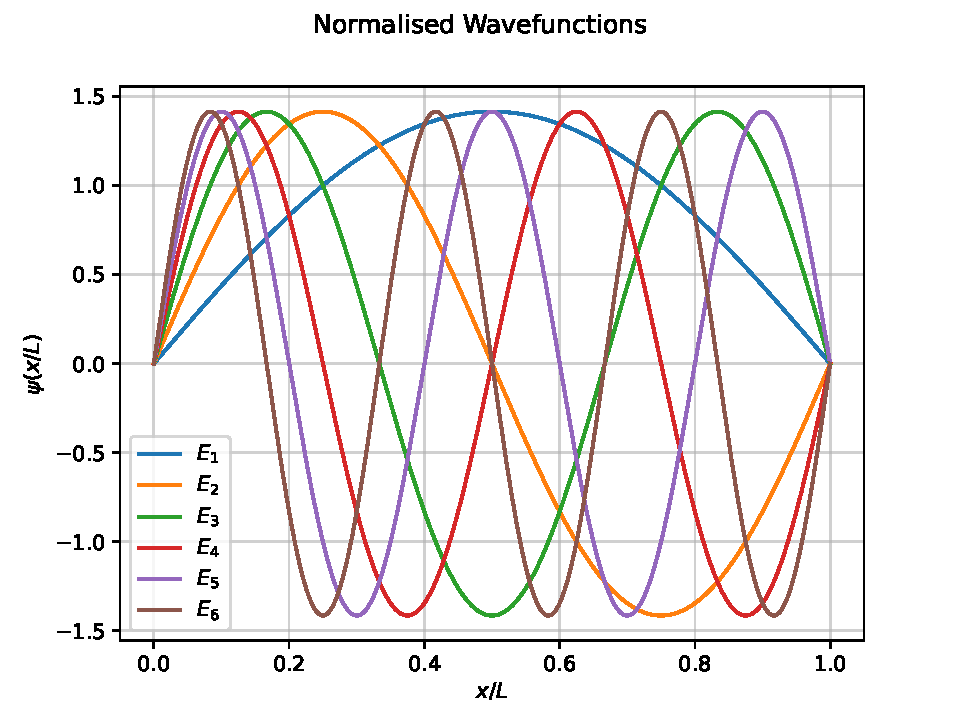
\includegraphics[width=0.38\textwidth]{Normalised Wavefunctions_nu.pdf}
            \end{tabular}   
        \end{tabular}
    \caption{\label{fig: square_well_results}This figure compares analytic and computational results for values of dimensionless energies $\varepsilon_n$ for the infinite square well potential well in the table on the left. On the right, the un-normalised wavefunctions are plotted above the normalised ones. In the upper centre, the error in the computed energies versus the analytic energies is plotted, note that the error is proportional to $n^2$. In the lower centre, $\sigma_{\tilde{x}}\sigma_{\tilde{p}}$ is plotted against $n$, showing that the uncertainty principle is obeyed, and the computed uncertainty relations agree with the analytic ones.}
\end{figure}
\subsection{Harmonic Potential}
\label{sec: harmonic_potential_results}


\begin{wrapfigure}{r}{0.35\textwidth}
    \centering
    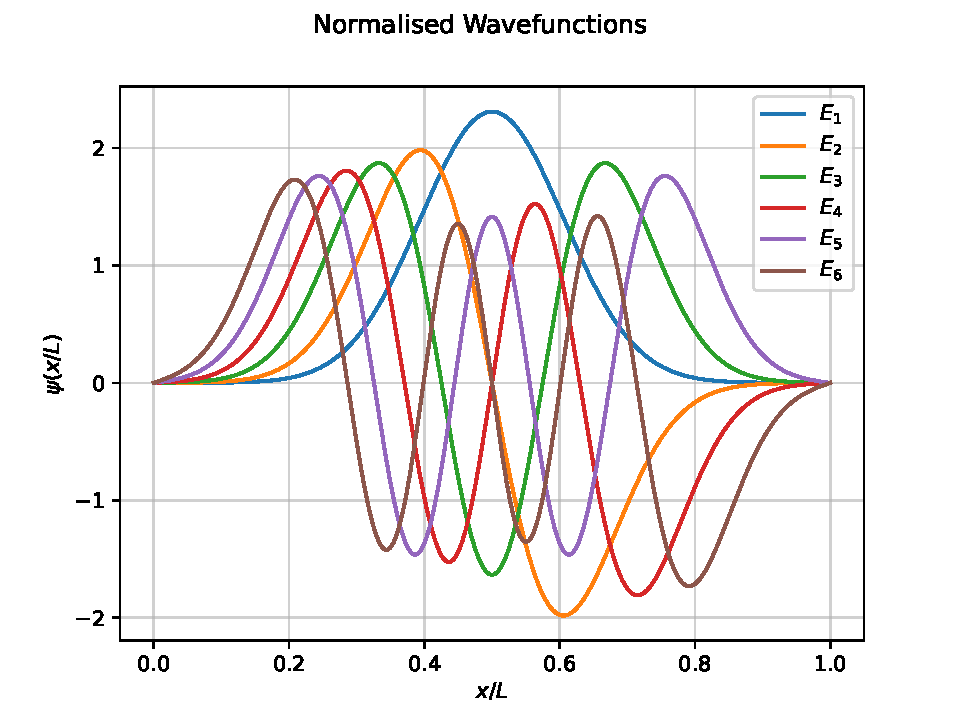
\includegraphics[width=0.35\textwidth]{Normalised Wavefunctions_harmonic_nu.pdf}
    \caption{\label{fig: harmonic_potential_wavefunctions}Normalised wavefunctions for the harmonic potential inside an infite potential well in the region.}
    
\end{wrapfigure}
The first result of the harmonic potential inside the infinite square well is the energy eigenvalues found by the shooting method, and their corresponding wavefunctions. The first 6 of these are plotted in figure \ref{fig: harmonic_potential_results}. The wavefunctions are normalised, and resemble somewhat Hermite polynomials, although they do not, however have any values outside of the defined region of the square well. From our definition of the harmonic potential inside the square well, we can reason that for large energy, $\varepsilon > 1$, the wavefunctions and energies behave as those of the simple infinite square well, and that for small energy $\varepsilon < 1$, the wavefunctions and energies behave as those of the harmonic oscillator. The reason for choosing $1$ as the boundary between these two regions is that this is the value of the potential at the point where it meets the well, as can be reasoned from Eq. \ref{eq: harmonic_potential}\\
\indent While they are included below, the explicit values of the energy eigenvalues for the harmonic potential are not the easiest way to see the transition from harmonic oscillator to bounded free particle. This is most easily seen by studying the difference between subsequent energies for the harmonic oscillator as in the lower left plot of figure \ref{fig: harmonic_potential_results}. It can be seen that by the point $n=11,12$, the difference between subsequent energies is increasing linearly, rather than staying constant, as it does for the harmonic oscillator. This agrees with the expected value $\varepsilon = 1$ for which the boundary between the two regions is defined.\\

\begin{figure}[h]
    \centering
    \begin{tabular}{cc}
        \multicolumn{2}{c}{
        \begin{tabular}{|p{0.02\textwidth}|p{0.045\textwidth}p{0.045\textwidth}p{0.045\textwidth}p{0.045\textwidth}p{0.045\textwidth}p{0.045\textwidth}p{0.045\textwidth}p{0.045\textwidth}p{0.045\textwidth}p{0.045\textwidth}p{0.045\textwidth}p{0.045\textwidth}p{0.045\textwidth}p{0.045\textwidth}p{0.045\textwidth}|}
            \hline
            $n$ & 1 & 2 & 3 & 4 & 5 & 6 & 7 & 8 & 9 & 10 & 11 & 12 & 13 & 14 & 15 \\
            $\varepsilon_n$ & -0.91 & -0.73 & -0.55 & -0.37 & -0.19 & -0.01 & 0.16 & 0.35 & 0.53 & 0.72 & 0.93 & 1.15 & 1.39 & 1.65 & 1.93 \\
            \hline
        \end{tabular}}\\
        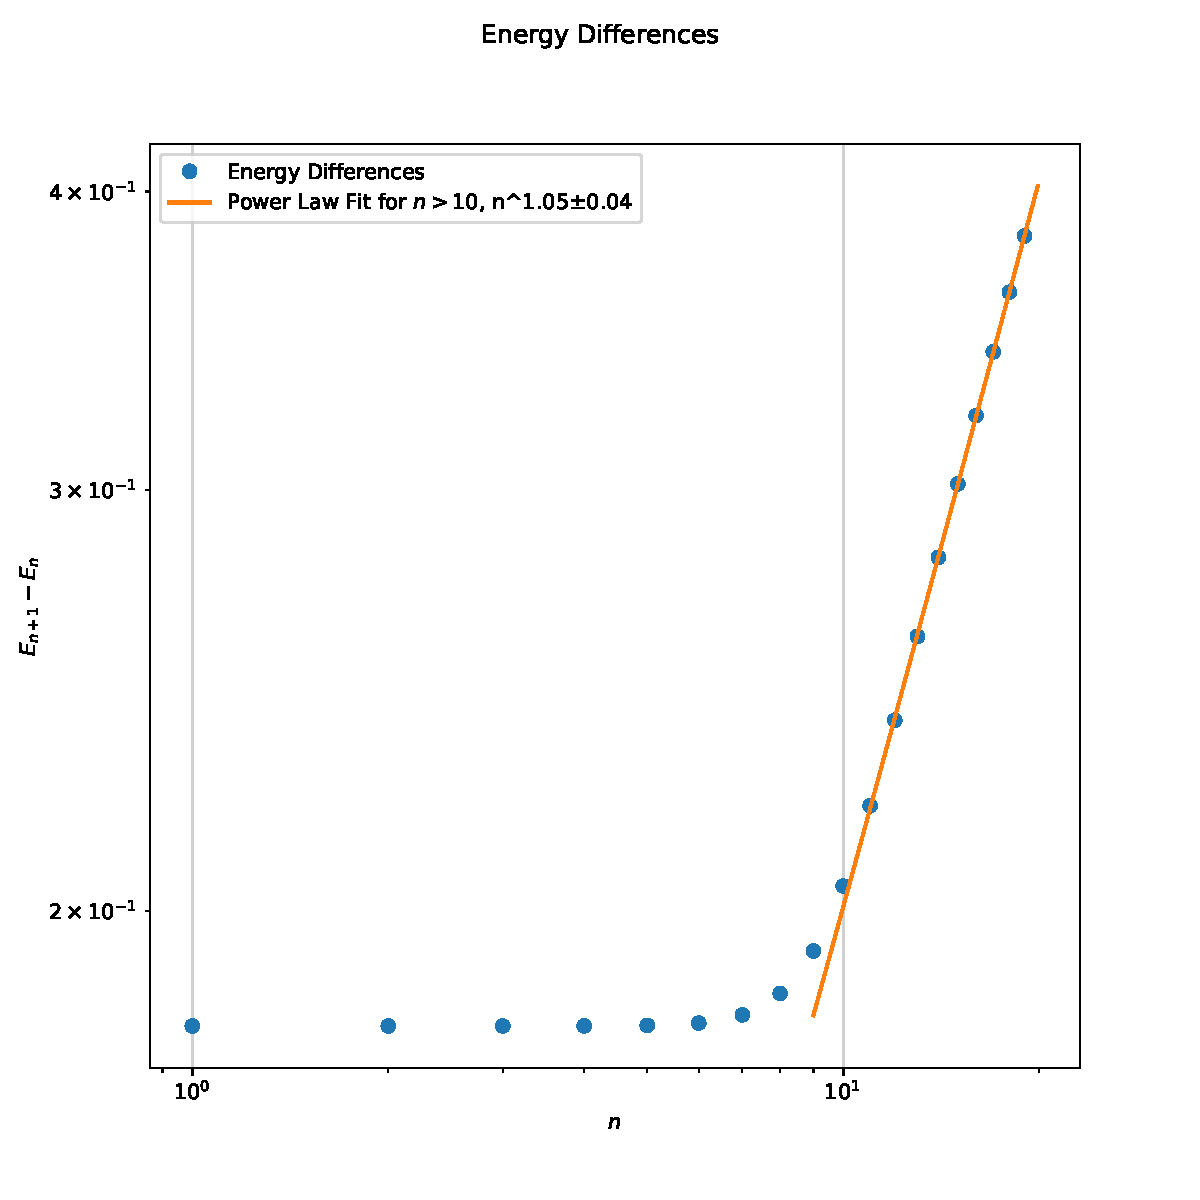
\includegraphics[width=0.4\textwidth]{energy_diffs_harmonic_nu.pdf}&
        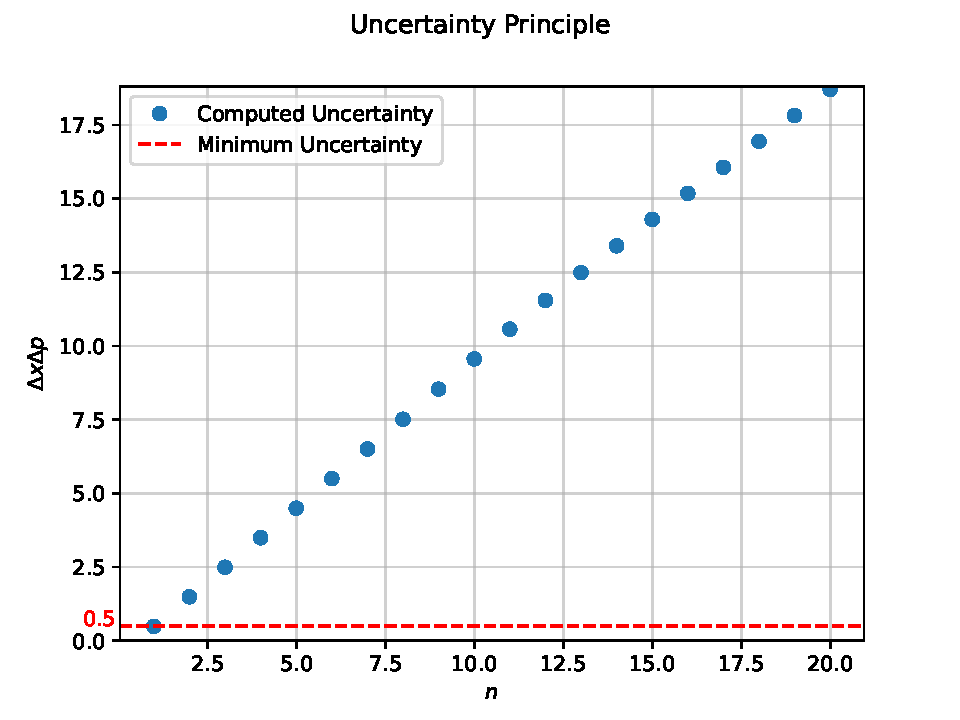
\includegraphics[width=0.4\textwidth]{uncertainty_principle_for_harmonic_nu.pdf}
    \end{tabular}
    \caption{\label{fig: harmonic_potential_results}At the top of this figure, the first 15 energy eigenvalues for the harmonic potential inside the infinite square well are shown up to two decimal places. The plot on the left shows the difference between subsequent energy eigenvalues, showing the transition from harmonic oscillator to free particle in a square well, by the change from linear to quadratic behaviour. The plot on the right shows the computed values of $\sigma_{\tilde{x}}\sigma_{\tilde{p}}$ against $n$, showing that the uncertainty principle is (approximately) obeyed.}
\end{figure}
\section{Conclusion}
In conclusion, it was found that the finite difference method, when used together with the shooting method, found, to a satisfactory degree of accuracy, the energy eigenvalues of the infinite square well potential (Eq. \ref{eq: square_well}), and the harmonic potential inside the infinite square well (Eq. \ref{eq: harmonic_potential}). Once found, the wavefunctions were normalised, and for both the potentials studied, the results satisfied the uncertainty principal approximately. It should be noted that the accuracy to which any computational value can be found is limited not only by the accuracy of the processes, but the precision of the computer with respect to floats.\\
\indent A particularly interesting result was the transition from harmonic oscillator to free particle in a square well, as seen in the lower left plot of figure \ref{fig: harmonic_potential_results}. When studying the data produced by the system, one can see that not only does the energy transition, but the wavefunctions, expectation values, and dispersions do also (Figures \ref{fig: means and dispersions for square well}, \ref{fig: means and dispersions for harmonic potential} in appendix).

\appendix
\begin{figure}
    \centering
    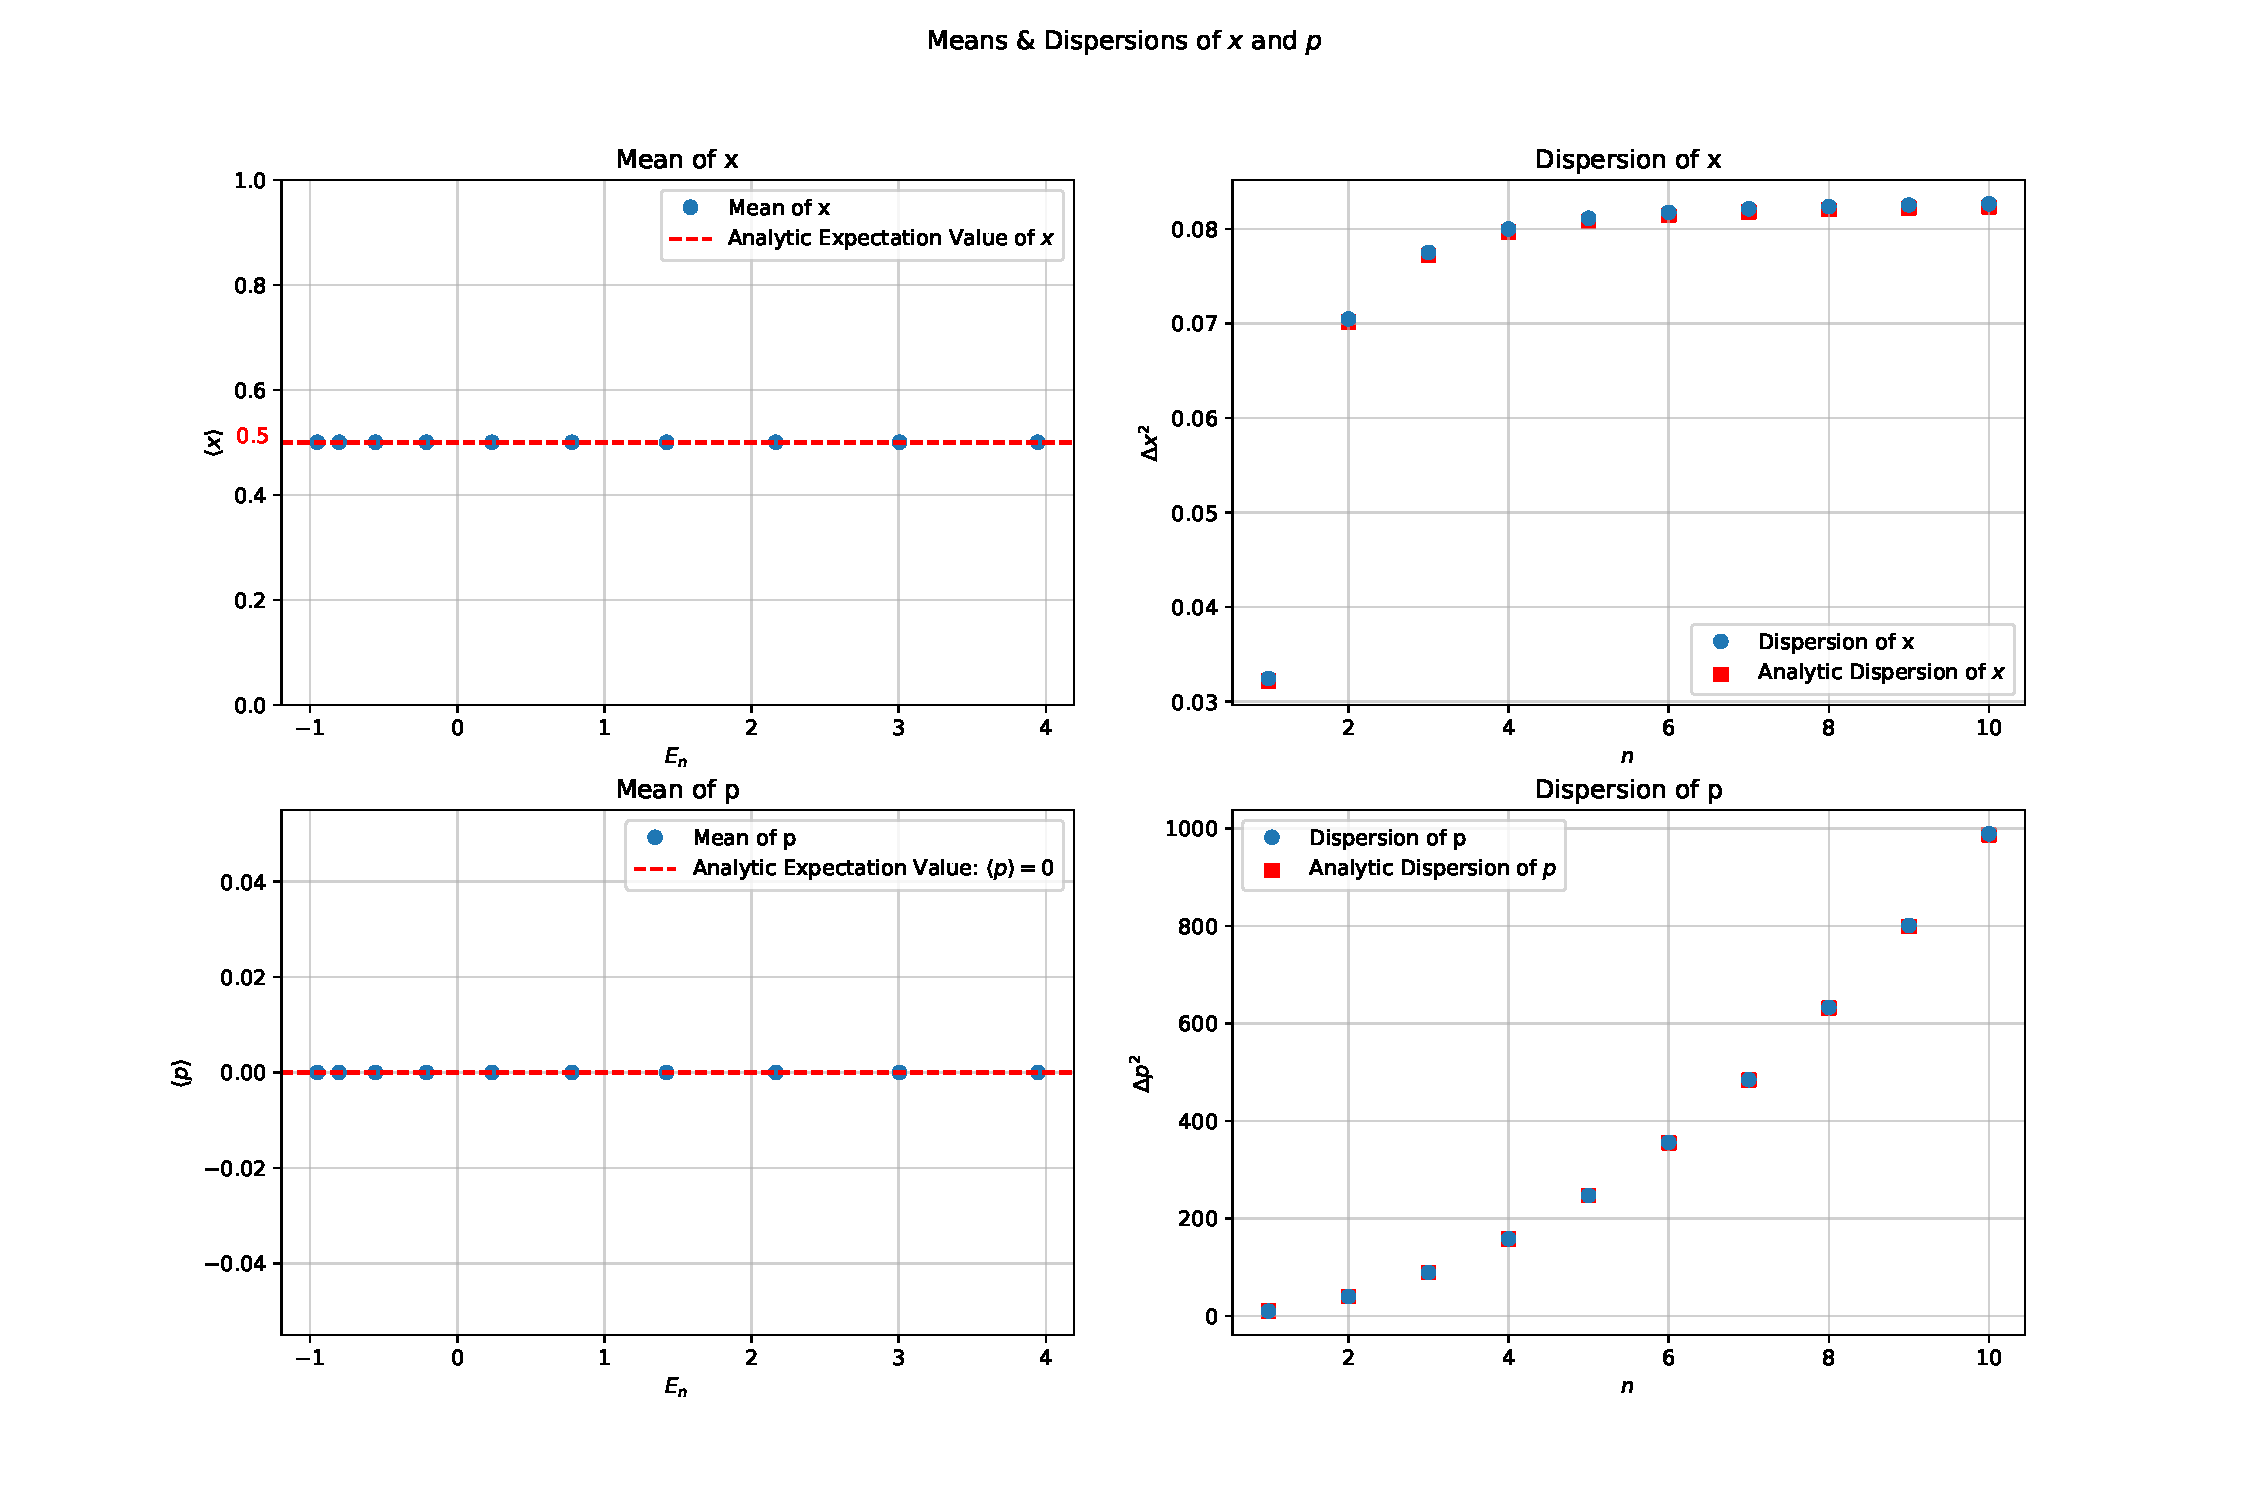
\includegraphics[width=0.8\textwidth]{means_and_dispersions_for_nu.pdf}
    \caption{\label{fig: means and dispersions for square well} The means and dispersions of the position and momentum operators and their squares for the infinite square well potential.}
\end{figure}
\begin{figure}
    \centering
    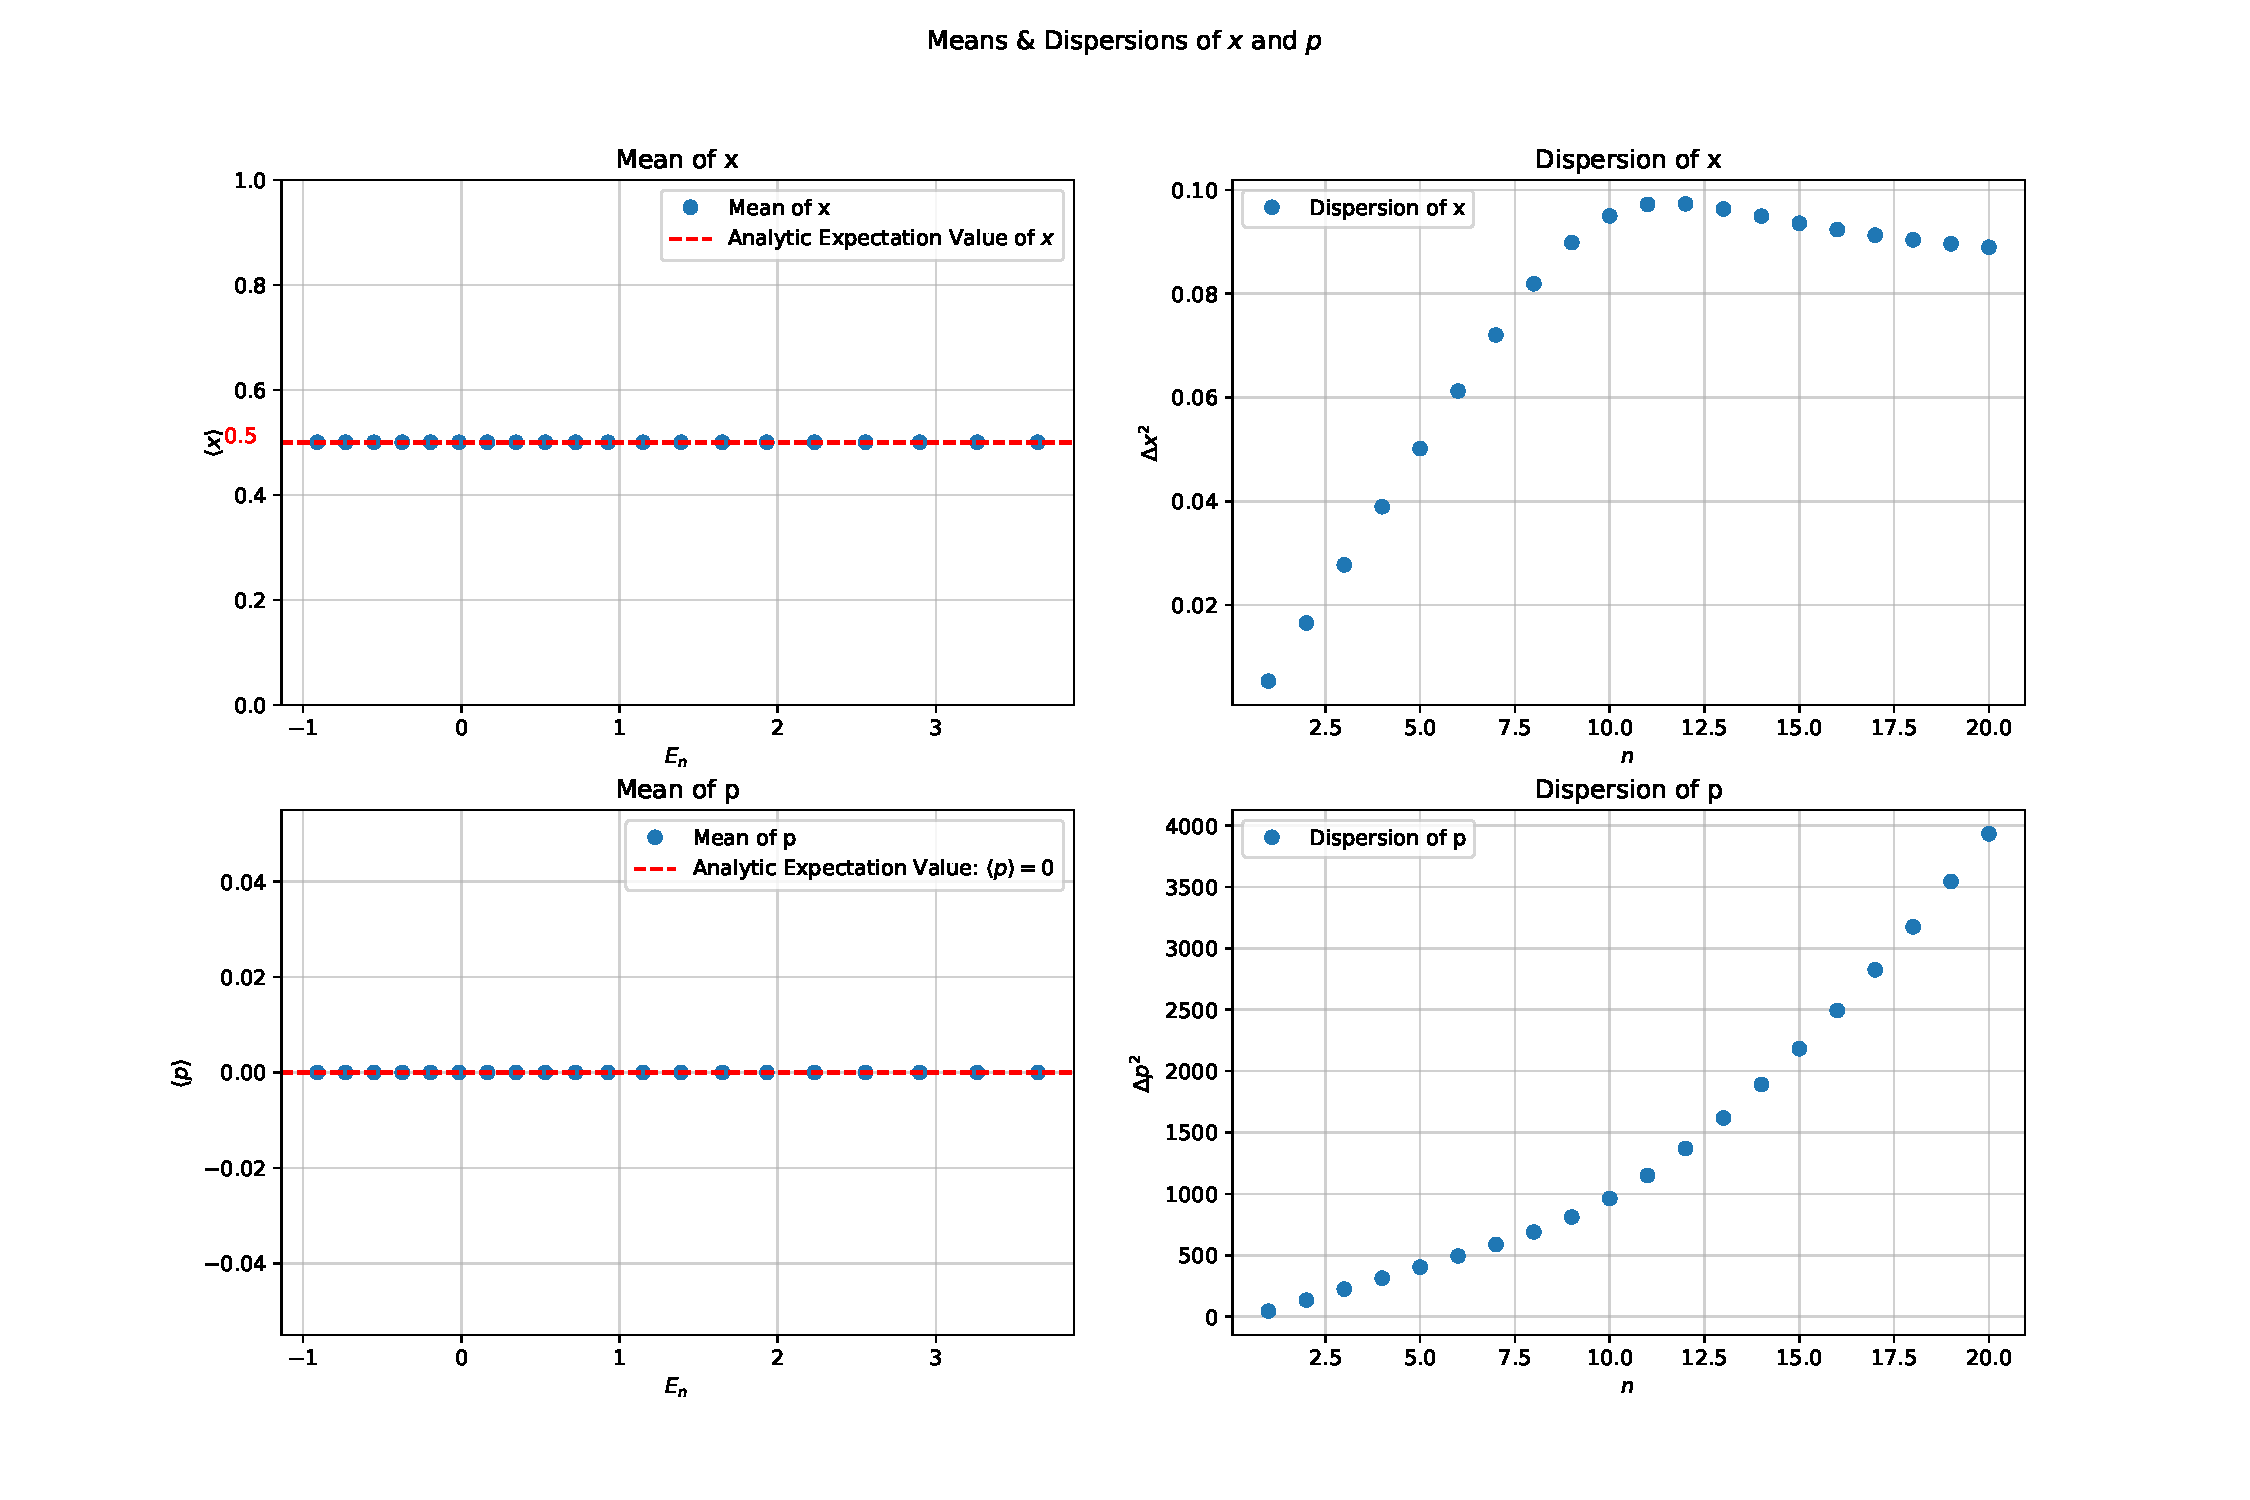
\includegraphics[width=0.8\textwidth]{means_and_dispersions_for_harmonic_nu.pdf}
    \caption{\label{fig: means and dispersions for harmonic potential} The means and dispersions of the position and momentum operators and their squares for the harmonic potential inside the infinite square well. Note the convergence of $\braket{x^2}$ to the same value for the harmonic potential as the square well in figure \ref{fig: means and dispersions for square well}}
\end{figure}
\bibliographystyle{plain}
\bibliography{references}

\end{document}